\section{Fine-Tuning Affordance for Dexterity}
\label{sec:method}

\begin{figure}[H]
\centering
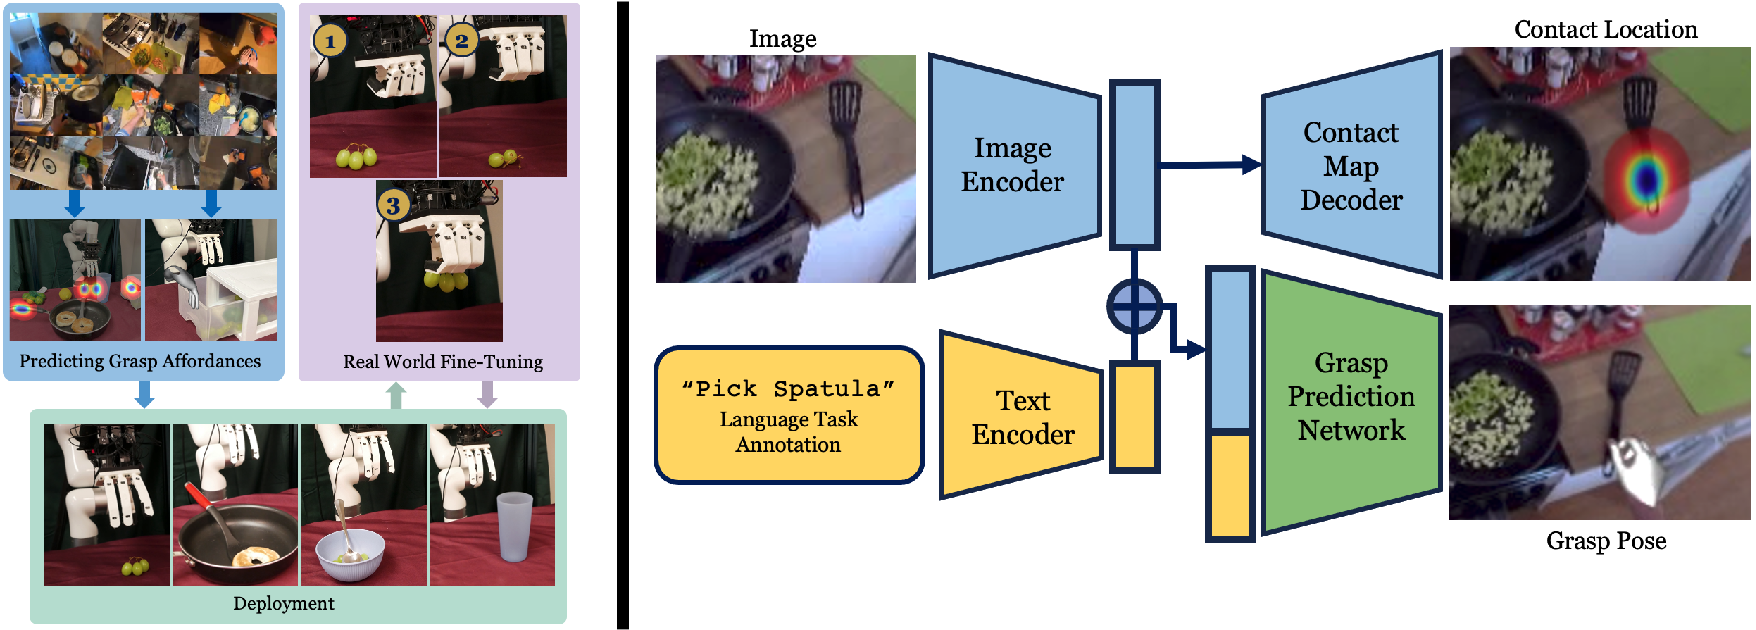
\includegraphics[width=\linewidth]{figs/method_overview.pdf}
\vspace{-0.2in}
  \caption{\small \textbf{Left:}  \ours consists of two phases: an affordance model that predicts grasp parameters followed by online fine-tuning with CEM. \textbf{Right:} Our affordance prediction setup predicts grasp location and pose.}
 \label{fig:aff_method}
 \vspace{-0.15in}
\end{figure}

The goal of \ours is to learn useful, dexterous manipulation in the real world that can generalize to many objects and scenarios.  \ours learns in the real-world and fine-tunes robot hand-to-object interaction in the real world using only a few samples. However, without any priors on what is useful behavior, the robot will explore the action space inefficiently. Especially with a high-dimensional robotic hand, we need a strong prior to effectively explore the real world. We train an affordance model on human videos to learn what are reasonable behaviors the robot should perform.  

\subsection{Learning grasping affordances}
\begin{figure}[t]
\centering
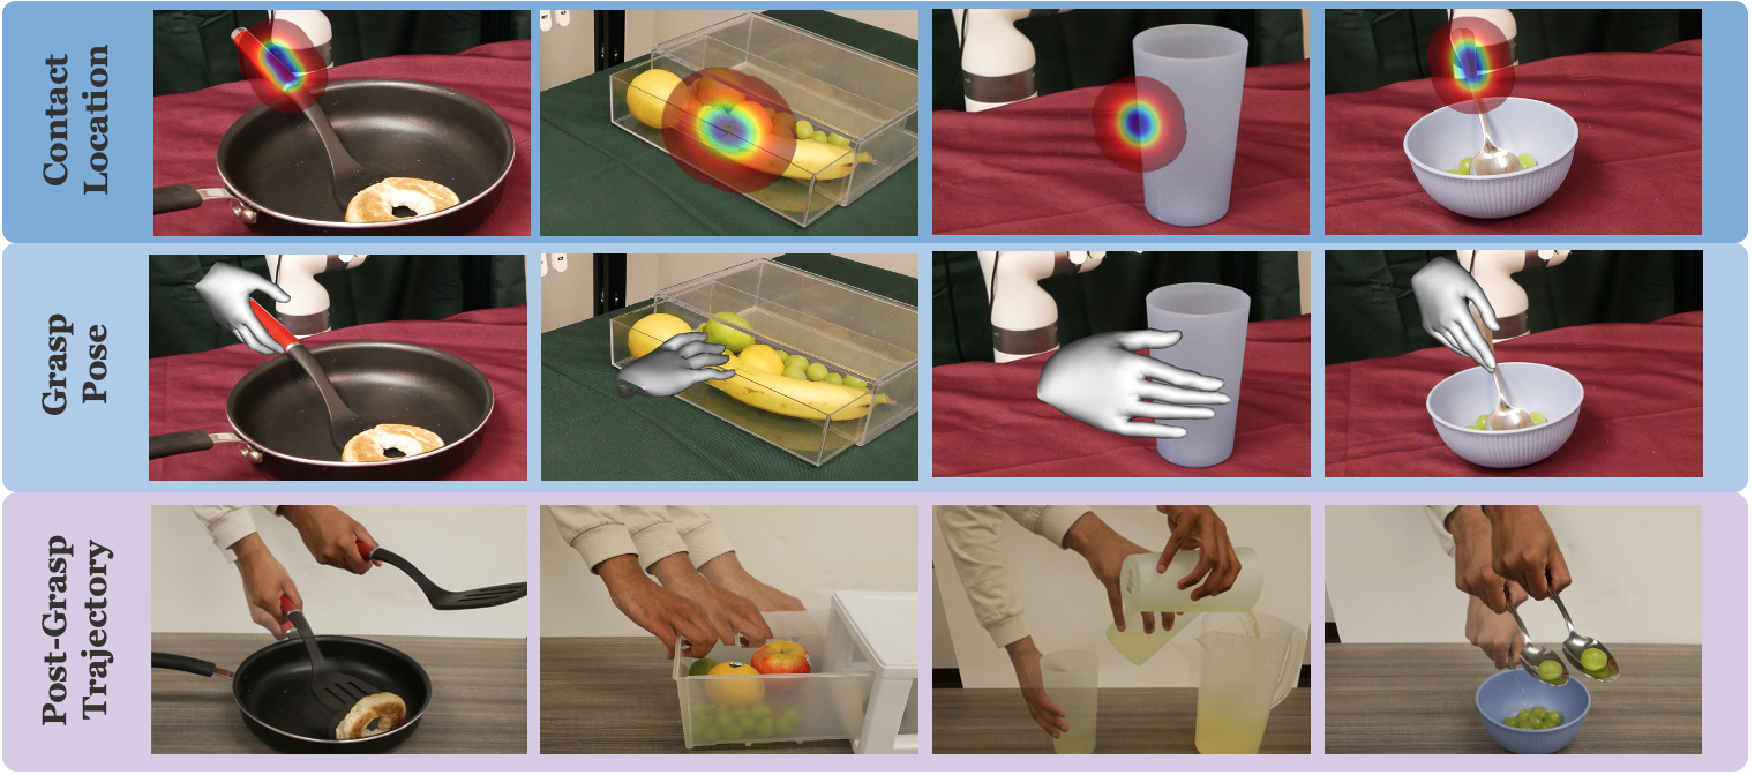
\includegraphics[width=\linewidth]{figs/aff_results.pdf}
\vspace{-0.2in}
  \caption{\small We produce three priors from human videos: the contact location (\textbf{top row}) and grasp pose (\textbf{middle row}) from the affordance prior; the post-grasp trajectory (\textbf{bottom row}) from a human demonstration of the task.}
 \label{fig:aff_results}
 \vspace{-0.15in}
\end{figure}


% \begin{wrapfigure}{l}{0.5\textwidth}
% \vspace{-0.3in}
% \begin{minipage}{\linewidth}
% \begin{algorithm}[H]
% \caption{\small Training affordances for \ours}\label{alg:cap}
% \begin{algorithmic}
% \small
% \REQUIRE Human videos $V_{1:K}$, task descriptions $T_{1:K}$, affordance model $f$. Human detection $f_\text{human}$ \citep{FrankMocap_2021_ICCV}. 

% \end{algorithmic}
% \label{algo:affordance}

% \end{algorithm}
% \end{minipage}
% \end{wrapfigure}


To learn from dexterous interaction in a sample efficient way, we use human hand motion as a prior for robot hand motion. We aim to answer the following: (1) What useful, actionable information can we extract from the human videos? (2) How can human motion be translated to the robot embodiment to guide the robot? In internet videos, humans frequently interact with a wide variety of objects. This data is especially useful in learning object affordances. Furthermore, one of the major obstacles in manipulating objects with few samples is accurately grasping the object. A model that can perform a strong grasp must learn \textit{where} and \textit{how} to grasp. Additionally, the task objective is important in determining object affordances--humans often grasp objects in different ways depending on their goal. Therefore, we extract three pieces of information from human videos: the grasp location, the human grasp pose, and the task.

Given a video clip $V = \{ v_1, v_2, \dots, v_T \} $, the first frame $v_t$ where the hand touches the object is found using a pre-trained, off-the-shelf hand-object detection model \cite{100doh}. Similar to previous approaches \cite{bahl2023affordances, hap, hoi, hotspots}, a set of contact points are extracted to fit a Gaussian Mixture Model (GMM) with centers $\mu = \{ \mu_1, \mu_2, \dots, \mu_k \}$.  Detic \cite{detic} is used to obtain a cropped image $v_1'$ containing just the object in the initial frame $v_1$ to condition the model. We use Frankmocap \cite{FrankMocap_2021_ICCV} to extract the hand grasp pose $P$ in the contact frame $v_t$ as MANO parameters. We also obtain the wrist orientation $\theta_\text{wrist}$ in the camera frame. This guides our prior to output wrist rotations and hand joint angles that produce a stable grasp. Finally, we acquire a text description $T$ describing the action occurring in $V$.

We extract affordances from three large-scale, egocentric datasets: Ego4D \cite{ego4d} for its large scale and the variety of different scenarios depicted, HOI4D \cite{hoi4d} for high-quality human-object interactions, and EPIC Kitchens \cite{EPICKITCHENS} for its focus on kitchen tasks similar to our robot's. We learn a task-conditioned affordance model $f$ that produces $(\hat{\mu}, \hat{\theta}_\text{wrist}, \hat{P}) = f(v_1', T)$. We predict $\hat{\mu}$ in similar fashion to \cite{bahl2023affordances}. First, we use a pre-trained visual model \cite{r3m} to encode $v_1'$ into a latent vector $z_v$. Then we pass $z_v$ through a set of deconvolutional layers to get a heatmap over $v_1'$ and use a spatial softmax to estimate $\hat{\mu}$.

To determine $\hat{\theta}_\text{wrist}$ and $\hat{P}$, we use $z_v$ and an embedding of the text description $z_T = g(T)$, where $g$ is the CLIP text encoder \cite{Clip}. Because transformers have seen success in encoding various multiple modes of input, we use a transformer encoder $\mathcal{T}$ to predict $\hat{\theta}_\text{wrist}, \hat{P} = \mathcal{T}(z_v, z_T)$. Overall, we train our model to optimize
\begin{align}
    \mathcal{L} = \lambda_\mu || \mu - \hat{\mu} ||_2 + \lambda_\theta || \theta_\text{wrist} - \hat{\theta}_\text{wrist} ||_2 + \lambda_P || P - \hat{P} ||_2
\end{align}


At test time, we generate a crop of the object using Segment-Anything \cite{kirillov2023segment} and give our model a task description. The model generates contact points on the object, and we take the average as our contact point. Using a depth camera, we can determine the 3D contact point to navigate to. While the model outputs MANO parameters \cite{MANO:SIGGRAPHASIA:2017} that are designed to describe human hand joints, we retarget these values to produce similar grasping poses on our robot hand in a similar manner to previous approaches \cite{handa2020dexpilot, sivakumar2022robotic}. In addition to the affordance model $f$, we collect one demo of the human doing the robot task (Figure~\ref{fig:aff_results}). This demo is used as a prior on the post-grasp trajectory.  We extract the task-specific wrist trajectory after the grasp using \cite{FrankMocap_2021_ICCV}. In the fine-tuning stage, we initialize the post-grasp trajectory with this human demonstration. Once we have this prior, how can the robot \textit{improve} upon it? 


\subsection{Fine-tuning via Interaction}

\begin{wrapfigure}{l}{0.55\textwidth}
\vspace{-0.3in}
\begin{minipage}{\linewidth}
\begin{algorithm}[H]
\caption{\small Fine-Tuning Procedure for \ours}\label{alg:cap}
\begin{algorithmic}
\small
\REQUIRE Task-conditioned affordance model $f$, task description $T$, post-grasp trajectory $\tau$, residual policy $\pi$. $E$ number of elites, $M$ number of warm-up episodes, $N$ total iterations. 

\FOR{$k = 1 \dots N$}
    \STATE $I_{k, 0} \gets $ initial image
    \STATE $\xi_k \gets f(I_{k, 0}, T)$
    \STATE $\epsilon_k = \pi(I_{k, 0}, \xi_k)$
    \STATE Execute grasp from $\xi_k + \epsilon_k$, then trajectory $\tau$
    \STATE Collect reward $R_k$; reset environment

    \IF{$k > M$}
        \STATE Order traj indices $i_1, i_2, \dots, i_k$ based on rewards
        \STATE $E \gets \{ \epsilon_{i_1}, \epsilon_{i_2}, \dots, \epsilon_{i_E} \} $
        \STATE Fit $\pi(.)$ as a VAE to $E$
    \ENDIF
\ENDFOR

\end{algorithmic}
\label{algo:finetune}

\end{algorithm}
\end{minipage}
\end{wrapfigure}


The affordance prior allows the robot to narrow down its learning behavior to a small subset of all possible behaviors. However, these affordances are not perfect and the robot will oftentimes still not complete the task.  This is partially due to morphology differences between the human and robot hands, inaccurate detections of the human hands, or differences in the task setup. In order to improve upon this, we practice in an online fashion to optimize the learned skills. 

Let the grasp location, wrist rotation and grasp pose, as well as the trajectory from our affordance prior be $\xi$. During training we sample noise $\epsilon \sim \mathcal{D}$ where $\mathcal{D}$ is initialized to $\mathcal{N}(0, \sigma^2)$ (for a small $\sigma$). We rollout a trajectory parameterized by $\xi + \epsilon$. We collect $R_i$, the reward for each $\xi_i = f(v_i) + \epsilon_i$ where $v_i$ is the image.  After an initial number of $M$ warmup episodes, we rank the rollouts based on $R_i$ and extract sampled noise from the elite trajectories $\{ \epsilon_{i_1}, \epsilon_{i_2}, \dots, \epsilon_{i_k} \}$. We fit $\mathcal{D}$ to the elite trajectories to improve the sampled noise. 

At test time, we could take the mean values of the top $N$ trajectories for the rollout policy.  However, this does not account for the appearance of different objects, previously unseen object configurations, or other properties in the environment. To account for this, we train a VAE \cite{SohnNIPS2015, rezende2014stochastic, rezende2014vae, kingma2013vae} to output residuals $\delta_j$ conditioned on an encoding of the initial image $\phi(I_{j, 0})$ and affordance model outputs $\xi_j$ from the top ten trajectories. We train an encoder $q(z | \delta_j, c_j)$ where $c_j = (\phi(I_{j, 0}), \xi_j)$, as well as a decoder $p(\delta_j | z, c_j)$. At test time, our residual policy $\pi (I_0, \xi)$ samples $z \sim \mathcal{N}(\mathbf{0}, \mathbf{I})$ and predicts $\hat{\delta} = p(z, (I_0, \xi))$. Then we rollout the trajectory determined by the parameters $\xi + \hat{\delta}$.
